\chapter{Arhitektura i dizajn sustava}
		
		\noindent Arhitekturu je moguće podijeliti na tri podsustava:
	\begin{itemize}
		\item 	Web poslužitelj
		\item 	Web aplikacija
		\item 	Baza podataka	
	\end{itemize}
		
		\underline{\textit{Web preglednik}} je program koji korisniku omogućuje pregled web-stranica i multimedijskog sadržaja vezanog uz njih. Korisnik putem web preglednika šalje zahtjev web poslužitelju te mu web preglednik kao interpreter prevodi web-stranicu i njezin sadržaj u format koji je korisniku razumljiv. \\
		\underline{\textit{Web poslužitelj}} temelj je rada web aplikacije te je njegov glavni zadatak omogućiti komunikaciju klijenta s aplikacijom. Komunikacija se ostvaruje preko protokola HTTP (engl. \textit{Hyper Text Transfer Protocol}), koji služi za prijenos informacija na webu. Web aplikacija se pokreće preko poslužitelja koji joj prosljeđuje zahtjev od strane korisnika. \\
		\underline{\textit{Web aplikacija}} služi za obradu korisničkih zahtjeva. Ovisno o zahtjevu, web aplikacija tijekom obrade zahtjeva pristupa bazi podataka te korisniku vraća odgovor u obliku HTML (engl. \textit{HyperText Markup Language}) dokumenta koji se prikazuje preko web preglednika. \\
		Codeshark web aplikacija bazirana je na programskom jeziku Python-u za razvoj \textit{backend}-a, zajedno s JavaScript-om uz biblioteku React za razvoj \textit{frontend}-a. Kao razvojno okruženje koristio se Microsoft Visual Studio. \\
		Arhitektura sustava temelji se na konceptu MVC-a (Model-View-Controller). Karakteristika MVC koncepta je nezavisan razvoj pojedinih dijelova aplikacije što za posljedicu ima jednostavnije ispitivanje kao i jednostavno razvijanje i dodavanje novih svojstava u sustav. \\
		
		\noindent MVC koncept sastoji se od:
		
		\begin{itemize}
			\item \textbf{Model} - Središnja komponenta sustava. Predstavlja dinamičke strukture podataka, neovisne o korisničkom sučelju. Izravno upravlja podacima, logikom i pravilima aplikacije. Ujedno i prima ulazne podatke od Controller-a.
			\item \textbf{View} - Bilo kakav prikaz podataka, poput grafa. Mogući su različiti prikazi iste informacije poput grafičkog ili tabličnog prikaza podataka.
			\item \textbf{Controller} - Prima ulaze i prilagođava ih za prosljeđivanje Model-u ili View-u. Upravlja korisničkim zahtjevima i temeljem njih izvodi daljnju interakciju s ostalim elementima sustava.
		\end{itemize}
		
				
		\section{Baza podataka}
		
		
		
		\noindent Za potrebe našeg sustava koristit  ćemo relacijsku bazu podataka koja svojom strukturom olakšava baratanju potrebnih podataka. Gradivna jedinka baze je relacija, odnosno tablica koja je definirana svojim imenom i skupom atributa. Zadaća baze podataka je brza i jednostavna pohrana, izmjena i dohvat podataka za daljnju obradu.
		Baza podataka ove aplikacije sastoji se od sljedećih entiteta:
		\begin{packed_item}
			\item Korisnik
			\item Natjecanje
			\item Zadatak
			\item Test-Primjeri
			\item Upload-Rjesenja
			\item Virtualno-Natjecanje
			\item Trofej
			\item Sudjeluje-Na
			\item Je-Osvojio
			\item Klasa-Natjecanja
			\item Sesija
		\end{packed_item}
		\subsection{Opis Tablica}
		\noindent \textbf{Korisnik} \space \space Ovaj entitet sadržava sve važne informacije o korisniku aplikacije.
		Sadrži atribute: Korisnikov ID, Korisničko ime, lozinku, ime, prezime, sliku profila, email, titulu, nivou prava, token, vrijeme generacije tokena i stanje aktivacije korisnika. Ovaj entitet u vezi je
		One-to-Many s entitetom Natjecanje preko ID-a korisnika (AutorID), u vezi One-to-Many s entitetom Zadatak preko ID-a korisnika (AutorID), u vezi One-to-Many s entitetom Sesija preko ID-a korisnika (KorisnikId), u vezi Many-to-Many s  Je-Osvojio preko ID-a korisnika, u vezi Many-to-Many s  Sudjeluje-na preko ID-a korisnika, u vezi One-to-Many s entitetom Upload-Rjesenja preko ID-a korisnika  te u vezi One-to-Many s entitetom VirtNatjecanje preko ID-a korisnika.
		
		
		\begin{longtblr}[
			label=none,
			entry=none
			]{
				width = \textwidth,
				colspec={|X[6,l]|X[6, l]|X[20, l]|}, 
				rowhead = 1,
			} %definicija širine tablice, širine stupaca, poravnanje i broja redaka naslova tablice
			\hline \multicolumn{3}{|c|}{\textbf{Korisnik}}	 \\ \hline[3pt]
			\SetCell{LightGreen}KorisnikId & SERIAL	&  jedinstveni indikator korisnika  	\\ \hline
			KorisnickoIme	& VARCHAR & identificirajuće ime korisnika  	\\ \hline 
			Lozinka	& VARCHAR & hash lozinke 	\\ \hline
			SlikaProfila	& VARCHAR &  slika profila korisnika 	\\ \hline 
			Ime & VARCHAR	&  ime korisnika		\\ \hline 
			Prezime & VARCHAR	&  prezime korisnika		\\ \hline 
			Email & VARCHAR & email korisnika  \\ \hline 
			Titula	& VARCHAR & prilagođena titula korisnika  	\\ \hline  
			NivouPrava	& INT & razina ovlasti korisnika  	\\ \hline
			Token	& VARCHAR & token napravljen za korisnika 	\\ \hline  
			Token Generiran	& TIMESTAMP & vrijeme kada je token generiran\\ \hline  
			Aktivan	& BOOLEAN & stanje verifikacije korisnika  	\\ \hline    
			
		\end{longtblr}
		
		\noindent \textbf{Natjecanje} \space \space Ovaj entitet sadržava sve važne informacije o održavanju natjecanja.
		Sadrži atribute:  ID Natjecanja, ime natjecanja, tekst natjecanja, vrijeme kraja natjecanja, vrijeme početka natjecanja, sliku trofeja, broj zadataka, ID autora natjecanja, ID klase natjecanja, ID trofeja. Ovaj entitet u vezi je	Many-to-One s entitetom Korisnik preko ID-a korisnika (AutorId), u vezi One-to-Many s entitetom Zadatak preko ID-a natjecanja , u vezi One-to-Many s  VirtNatjecanje preko ID-a natjecanja, u vezi One-to-One s  entitetom Trofej preko ID-a trofeja te u vezi Many-to-One s entitetom IDKlasaNatjecanja preko ID-a klase natjecanja.
		
		
		\begin{longtblr}[
			label=none,
			entry=none
			]{
				width = \textwidth,
				colspec={|X[6,l]|X[6, l]|X[20, l]|}, 
				rowhead = 1,
			} %definicija širine tablice, širine stupaca, poravnanje i broja redaka naslova tablice
			\hline \multicolumn{3}{|c|}{\textbf{Natjecanje}}	 \\ \hline[3pt]
			\SetCell{LightGreen}NatjecanjeId & SERIAL	&  jedinstveni indikator natjecanja  	\\ \hline
			ImeNatjecanja	& VARCHAR & identificirajuće ime natjecanja  	\\ \hline 
			Tekst Natjecanja	& VARCHAR & sadržaj teksta natjecanja 	\\ \hline
			VrijemeKraj	& TIMESTAMP & vrijeme završetka natjecanja 	\\ \hline 
			VrijemePoc & TIMESTAMP	&  vrijeme početka natjecanje		\\ \hline 
			SlikaTrofeja & VARCHAR	&  sličica trofeja		\\ \hline 
			BrojZadataka & INT & broj zadataka u natjecanju  \\ \hline 
			Slug & VARCHAR & slug verzija imena natjecanja  \\ \hline
			\SetCell{LightBlue} AutorId	& INT & autorov Korisnik ID (korisnik.KorisnikID) 	\\ \hline  
			\SetCell{LightBlue} ID Klase Natjecanja & INT & ID Klase Natjecanja (klasanatjecanja.IdKlaseNatjecanja)  	\\ \hline  
			\SetCell{LightBlue} TrofejID	& INT & Trofej ID (trofej.TrofejID)   	\\ \hline 
		\end{longtblr}
		
		\noindent \textbf{Zadatak} \space \space Ovaj entitet sadržava sve važne informacije o zadacima.
		Sadrži atribute:  Zadatak ID, ime zadatka, tekst zadatka, bodovi zadatka, maksimalno vrijeme izvršavanja zadatka, privatnost zadatka, slug naziv zadatka, id autora , id natjecanja(opcionalno). Ovaj entitet u vezi je	Many-to-One s entitetom Korisnik preko ID-a korisnika (AutorID), u vezi Many-to-One s entitetom Natjecanje preko ID-a natjecanja , u vezi One-to-Many s  TestPrimjeri preko ID-a zadatka  te u vezi One-to-Many s  entitetom UploadRjesenja preko ID-a zadatka.
		
		\begin{longtblr}[
			label=none,
			entry=none
			]{
				width = \textwidth,
				colspec={|X[6,l]|X[6, l]|X[20, l]|}, 
				rowhead = 1,
			} %definicija širine tablice, širine stupaca, poravnanje i broja redaka naslova tablice
			\hline \multicolumn{3}{|c|}{\textbf{Zadatak}}	 \\ \hline[3pt]
			\SetCell{LightGreen}ZadatakId & SERIAL	&  jedinstveni indikator zadatka  	\\ \hline
			ImeZadatka	& VARCHAR & identificirajući naziv zadatka  \\ \hline
			Bodovi	& INT & broj bodova(težina 1-5)	\\ \hline
			MaxVrijeme Izvrs	& NUMERIC &  maksimalno vrijeme izvršavanja programa 	\\ \hline 
			TekstZadatka & VARCHAR	&  sadržaj teksta zadatka		\\ \hline 
			Privatnost & BOOLEAN	&  stanje privatnosti zadatka	\\ \hline 
			Slug & VARCHAR & slug verzija naziva zadatka  \\ \hline 
			\SetCell{LightBlue} AutorId	& INT & autorov Korisnik ID (korisnik.KorisnikId)  	\\ \hline  
			\SetCell{LightBlue} NatjecanjeId & INT &(opcionalno) Natjecanje ID (natjecanje.NatjecanjeId)  	\\ \hline  
			
		\end{longtblr}
		
		\noindent \textbf{Test Primjeri} \space \space Ovaj entitet sadržava sve važne informacije o testnim primjerima za zasebne zadatke.
		Sadrži atribute:  Zadatak ID, ulaz testa, izlaz testa. Ovaj entitet u vezi je	Many-to-One s entitetom Zadatak preko ID-a zadatka.
		
		\begin{longtblr}[
			label=none,
			entry=none
			]{
				width = \textwidth,
				colspec={|X[6,l]|X[6, l]|X[20, l]|}, 
				rowhead = 1,
			} %definicija širine tablice, širine stupaca, poravnanje i broja redaka naslova tablice
			\hline \multicolumn{3}{|c|}{\textbf{TestPrimjeri}}	 \\ \hline[3pt]
			\SetCell{LightGreen}Ulaz & VARCHAR	&  ulaz testa  	\\ \hline
			\SetCell{LightGreen}ZadatakId	& INT & Zadatak ID (zadatak.ZadatakId)  	\\ \hline 
			Izlaz	& VARCHAR & željeni izlaz testa	\\ \hline
			
		\end{longtblr}
		
		\noindent \textbf{Upload Rjesenja} \space \space Ovaj entitet sadržava sve informacije koje su bitne oko uploada rješenja na zadatak.
		Sadrži atribute:  Zadatak ID, korisnikov id, vrijeme predaje rješenja, predano rješenje, prolaznost, prosječno vrijeme izvršavanja, aktivnost natjecanja. Ovaj entitet u vezi je	Many-to-One s entitetom Korisnik preko ID-a korisnika  te u vezi Many-to-One s entitetom Zadatak preko ID-a zadatka.
		
		
		\begin{longtblr}[
			label=none,
			entry=none
			]{
				width = \textwidth,
				colspec={|X[6,l]|X[6, l]|X[20, l]|}, 
				rowhead = 1,
			} %definicija širine tablice, širine stupaca, poravnanje i broja redaka naslova tablice
			\hline \multicolumn{3}{|c|}{\textbf{UploadRjesenja}}	 \\ \hline[3pt]
			\SetCell{LightGreen}VrijemePredaje & TIMESTAMP	&  vrijeme predaje rješenja  	\\ \hline
			\SetCell{LightGreen} KorisnikId	& INT & Korisnik ID (korisnik.KorisnikId)  	\\ \hline 
			\SetCell{LightGreen} ZadatakId	& INT & Zadatak ID (zadatak.ZadatakId)  	\\ \hline
			Predano Rjesenje	& VARCHAR &  datoteka koju je predao korisnik	\\ \hline 
			Prolaznost & NUMERIC	&  posto riješenosti primjera zadataka		\\ \hline 
			ProsjVrijeme Izvrs & NUMERIC	&  prosječno vrijeme izvršavanja po primjeru		\\ \hline 
			 
		\end{longtblr}
		
		\noindent \textbf{Virtualno Natjecanje} \space \space Ovaj entitet sadržava sve važne informacije o Virtualnim natjecanjima.
		Sadrži atribute:  Korisnikov ID, ID natjecanja, ID random zadatka težine 2, ID random zadatka težine 3, ID random zadatka težine 4 te ID random zadatka težine 5. Ovaj entitet u vezi je	Many-to-One s entitetom Korisnik preko ID-a korisnika, u vezi Many-to-One s entitetom Natjecanje preko ID-a natjecanja te u 4 veze Many-to-One s entitetom Zadatak preko ID-ova zadataka.
		
		
		\begin{longtblr}[
			label=none,
			entry=none
			]{
				width = \textwidth,
				colspec={|X[6,l]|X[6, l]|X[20, l]|}, 
				rowhead = 1,
			} %definicija širine tablice, širine stupaca, poravnanje i broja redaka naslova tablice
			\hline \multicolumn{3}{|c|}{\textbf{VirtNatjecanje}}	 \\ \hline[3pt]
			\SetCell{LightGreen}VirtNatjecanje Id & SERIAL	& identifikacijski broj virtualnog natjecanja\\ 	\hline
			Vrijeme Kreacije & TIMESTAMP & vrijeme kreacije virtualnog natjecanja \\ \hline
			Zadaci	& INTEGER[] & (Opcionalno) array svih random odaberenih zadataka \\ \hline
			\SetCell{LightBlue}NatjecanjeId	& INT & (Opcionalno) Natjecanje ID (natjecanje.NatjecanjeId) \\ \hline
			\SetCell{LightBlue}KorisnikId & INT	&  Korisnik ID  (korisnik.KorisnikId)	\\ 	\hline
			 
		\end{longtblr}
		
		
		\noindent \textbf{Trofej} \space \space Ovaj entitet sadržava sve važne informacije o trofejima.
		Sadrži atribute:  Trofej ID, ime trofeja, slika trofeja. Ovaj entitet u vezi je	Many-to-One s entitetom Korisnik preko ID-a korisnika, u vezi One-to-Many s entitetom Natjecanje preko ID-a trofeja te u vezi Many-to-Many s Je-Osvojio preko ID-a trofeja.
		
		\begin{longtblr}[
			label=none,
			entry=none
			]{
				width = \textwidth,
				colspec={|X[6,l]|X[6, l]|X[20, l]|}, 
				rowhead = 1,
			} %definicija širine tablice, širine stupaca, poravnanje i broja redaka naslova tablice
			\hline \multicolumn{3}{|c|}{\textbf{Trofej}}	 \\ \hline[3pt]
			\SetCell{LightGreen}TrofejID & SERIAL	&  jedinstveni indikator trofeja  	\\ \hline
			ImeTrofeja	& VARCHAR & ime trofeja	\\ \hline 
			SlikaTrofeja	& VARCHAR & slika trofeja	\\ \hline
			
		\end{longtblr}
		
		\noindent \textbf{Sudjeluje Na} \space \space Ovaj entitet sadržavi listu svih sudjelovanja korisnika na natjecanjima.
		Sadrži atribute:  Korisnik ID, Natjecanje ID.
		
		\begin{longtblr}[
			label=none,
			entry=none
			]{
				width = \textwidth,
				colspec={|X[6,l]|X[6, l]|X[20, l]|}, 
				rowhead = 1,
			} %definicija širine tablice, širine stupaca, poravnanje i broja redaka naslova tablice
			\hline \multicolumn{3}{|c|}{\textbf{SudjelujeNa}}	 \\ \hline[3pt]
			\SetCell{LightGreen}KorisnikId & INT	&  Korisnik ID (korisnik.KorisnikId)	\\ \hline
			\SetCell{LightGreen}NatjecanjeId	& INT & Natjecanje ID (natjecanje.NatjecanjeId)	\\ \hline 
			
		\end{longtblr}
		
		\noindent \textbf{Je Osvojio} \space \space Ovaj entitet sadržava listu svih korisnika s osvojenim peharima.
		Sadrži atribute:  Korisnik ID, Trofej ID. Ovaj entitet u vezi je One-To-Many s entitetom Natjecanje preko ID-a klase natjecanja.
		
		\begin{longtblr}[
			label=none,
			entry=none
			]{
				width = \textwidth,
				colspec={|X[6,l]|X[6, l]|X[20, l]|}, 
				rowhead = 1,
			} %definicija širine tablice, širine stupaca, poravnanje i broja redaka naslova tablice
			\hline \multicolumn{3}{|c|}{\textbf{JeOsvojio}}	 \\ \hline[3pt]
			\SetCell{LightGreen}KorisnikId & INT	&  Korisnik ID (korisnik.KorisnikId)  	\\ \hline
			\SetCell{LightGreen}TrofejId	& INT & Trofej ID (trofej.TrofejId)  	\\ \hline 
			
		\end{longtblr}
		
		
		\noindent \textbf{Klasa Natjecanja} \space \space Ovaj entitet sadržava sve informacije o klasi natjecanja.
		Sadrži atribute:   ID klase natjecanja, naziv klase natjecanja.
		
		
		
		
		
		\begin{longtblr}[
			label=none,
			entry=none
			]{
				width = \textwidth,
				colspec={|X[6,l]|X[6, l]|X[20, l]|}, 
				rowhead = 1,
			} %definicija širine tablice, širine stupaca, poravnanje i broja redaka naslova tablice
			\hline \multicolumn{3}{|c|}{\textbf{KlasaNatjecanja}}	 \\ \hline[3pt]
			\SetCell{LightGreen}IdKlase Natjecanja & INT	&  jedinstveni indikator klase natjecanje  	\\ \hline
			NazivKlase Natjecanja	& VARCHAR & naziv klase natjecanja 	\\ \hline 
			
		\end{longtblr}
	
		\noindent \textbf{Sesija} \space \space Ovaj entitet sadržava sve informacije o korisničkoj sesiji.
		Sadrži atribute:  Sesija ID, Pocetak sesije, korisnikov ID.
		
		
		
		
		
		\begin{longtblr}[
			label=none,
			entry=none
			]{
				width = \textwidth,
				colspec={|X[6,l]|X[6, l]|X[20, l]|}, 
				rowhead = 1,
			} %definicija širine tablice, širine stupaca, poravnanje i broja redaka naslova tablice
			\hline \multicolumn{3}{|c|}{\textbf{Sesija}}	 \\ \hline[3pt]
			\SetCell{LightGreen}SesijaId & VARCHAR	&  jedinstveni indikator sesije 	\\ \hline
			PocetakSesije	& TIMESTAMP & timestamp pocetka sesije 	\\ \hline 
			\SetCell{LightBlue}KorisnikId & INT & id vlasnika sesije (Korisnik.KorisnikId) \\ \hline
			
		\end{longtblr}
		
		
		
		\subsection{Dijagram baze podataka}
		\begin{figure}[H]
			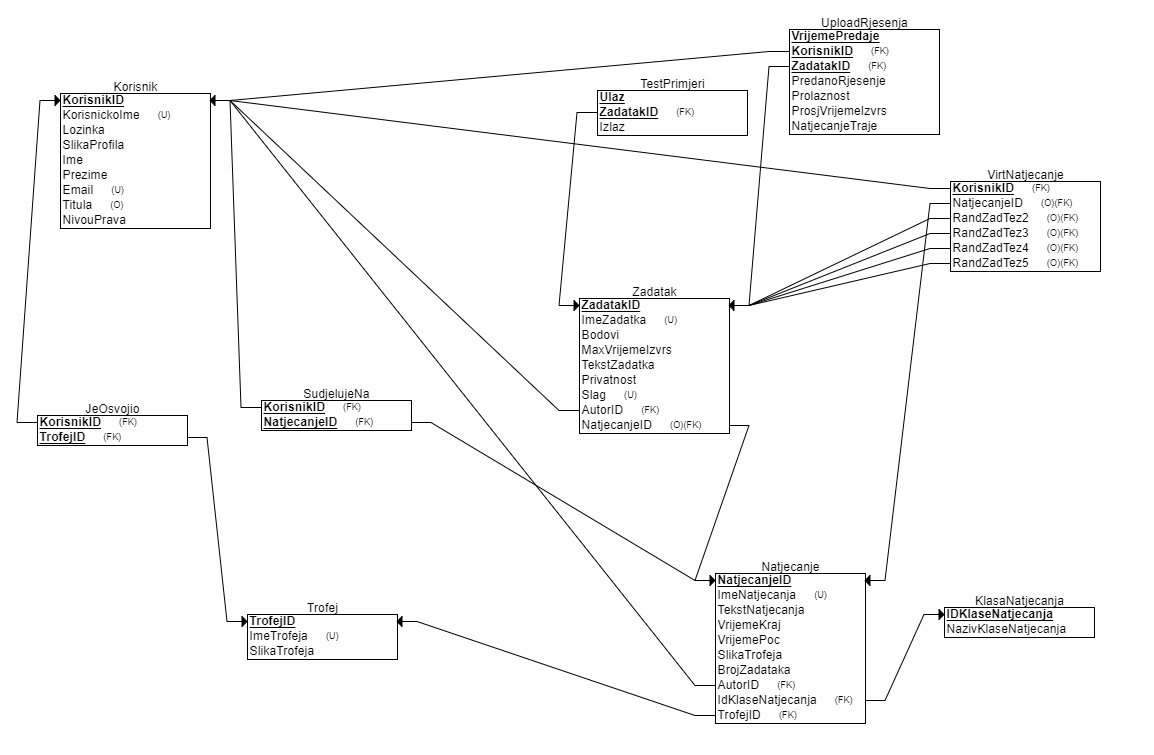
\includegraphics[width=\textwidth]{slike/RelacijskaShema.PNG} %veličina u odnosu na širinu linije
			\caption{E-R dijagram baze podataka}
			\label{fig:RelacijskaShema} %label mora biti drugaciji za svaku sliku
		\end{figure}
		
		\eject
			
			
		\section{Dijagram razreda}
			Na slici 4.2. vidimo osnovni model UML dijagrama koji prikazuje osnovne klase koje koristimo na backendu.
				
			Trenutni dijagram razreda opisuje izgled klasa i njihovih metoda koje će nam biti potrebne u projektu. 
			Trenutno pošto imamo registraciju, ulogiravanje i validaciju, koristimo samo klasu Korisnik te njene metode. 
			Imamo privatnu metodu koja se zove \verb*|__get_id()| preko koje dobivamo korisnikid iz baze podataka,
			zato što je to metoda koja dohvaća privatni ključ te ne želimo da korisnik ikad ima pristup tome.
			Tu metodu trenutno ne koristimo previše već će biti jako korisna kasnije u konekcijama s instancama ostalim
			klasa prilikom dobivanja informacija iz ostalih tablica baze podataka. Kao što se vidi, svaka klasa ima 
			konstruktor \verb*|__init__()| te primaju informacije koje su identične onima iz njihovih modela iz baze podataka.

			\begin{figure}[H]
				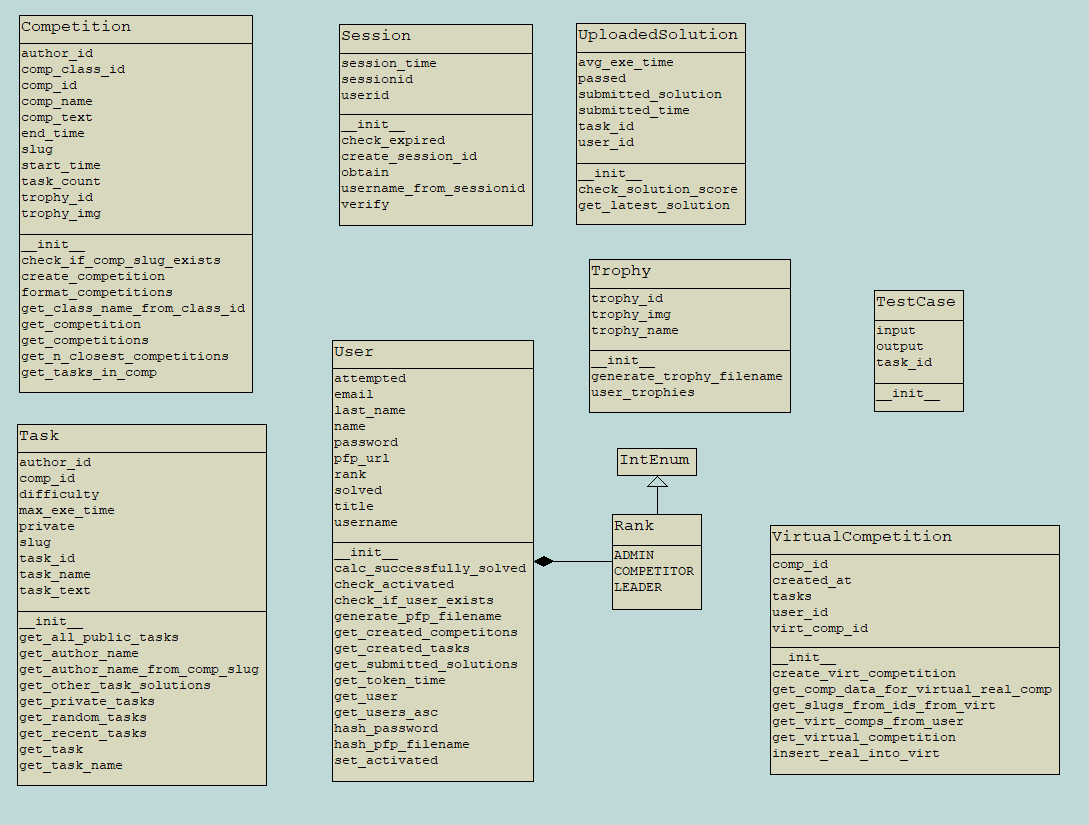
\includegraphics[width=\textwidth]{slike/DijagramRazreda.png} %veličina u odnosu na širinu linije
				\caption{Dijagram razreda}
				\label{fig:DijagramRazreda} %label mora biti drugaciji za svaku sliku
			\end{figure}	
			

			Budući da radimo u programskom jeziku Python, ne možemo lako prikazati Data Transfer objects.
			Međutim, prilikom registracije, sve informacije koje dobivamo s frontenda prosljeđujemo u konstruktor
			Korisnik. Kasnije, prilikom login-a, preko korisničkog imena dobivamo podatke iz baze te izrađujemo instancu Korisnik.
			S tim Korisnikom možemo baratati pomoću njegovih podataka. Tražimo iz baze podataka je li aktiviran te odgovara li
			hash unesene lozinke hashu lozinke koja je spremljena u bazu podataka, tj. u instanci Korisnik.

			Naša klasa Korisnik se zapravo referira i na voditelja i na administratora. Oni svi imaju identične podatke te duplikacija koda
			nije potrebna. Velika razlika je samo u njihovom podatku NivouPrava o kojem će ovisiti kakve ovlasti na stranici ima.
			To će također biti funkcija koju će biti privatna. Voditelj će za razliku od natjecatelja imati pristup stranicama
			za  kreiranje zadataka te stvaranju natjecanja. Administrator će uz to sve moći uređivati ovlasti svih korisnika te će pomoću toga imati mogućnost potvrditi voditelja što će biti na posebnoj stranici.



			
			
			
			\eject
		
		\section{Dijagram stanja}
			
		
			Dijagram stanja prikazuje stanja objekta te prijelaze iz jednog stanja u drugo temeljene na događajima. Na slici 4.3 prikazan je dijagram stanja za registriranog natjecatelja. Nakon prijave, natjecatelju se prikazuje početna stranica na kojoj može otiči na stranicu zadataka. Klikom na odabrani zadatak on unosi svoj programski kod koji se šalje na provjeru te dobiva rezultate. Također, može otiči na stranicu natjecanja gdje mi se nudi sva bivša,trenutna i buduća natjecanja. Klikom na natjecanje ga vodi na stranicu tog natjecanje gdje ga ima opciju pokrenuti. Ovisno o statusu trajanja natjecanje, pokreće se različita instanca natjecanja. Na toj instanci se prikazuju zadaci koje je moguće riješiti u ograničenom vremenu. Uz stranice zadataka i natjecanja, natjecatelj uvijek može pristupiti stranici vlastitog profila na kojoj može uređivati svoje podatke, te stranici ostalih članova s koje može gledati profile ostalih korisnika. 
			
			\begin{figure}[H]
				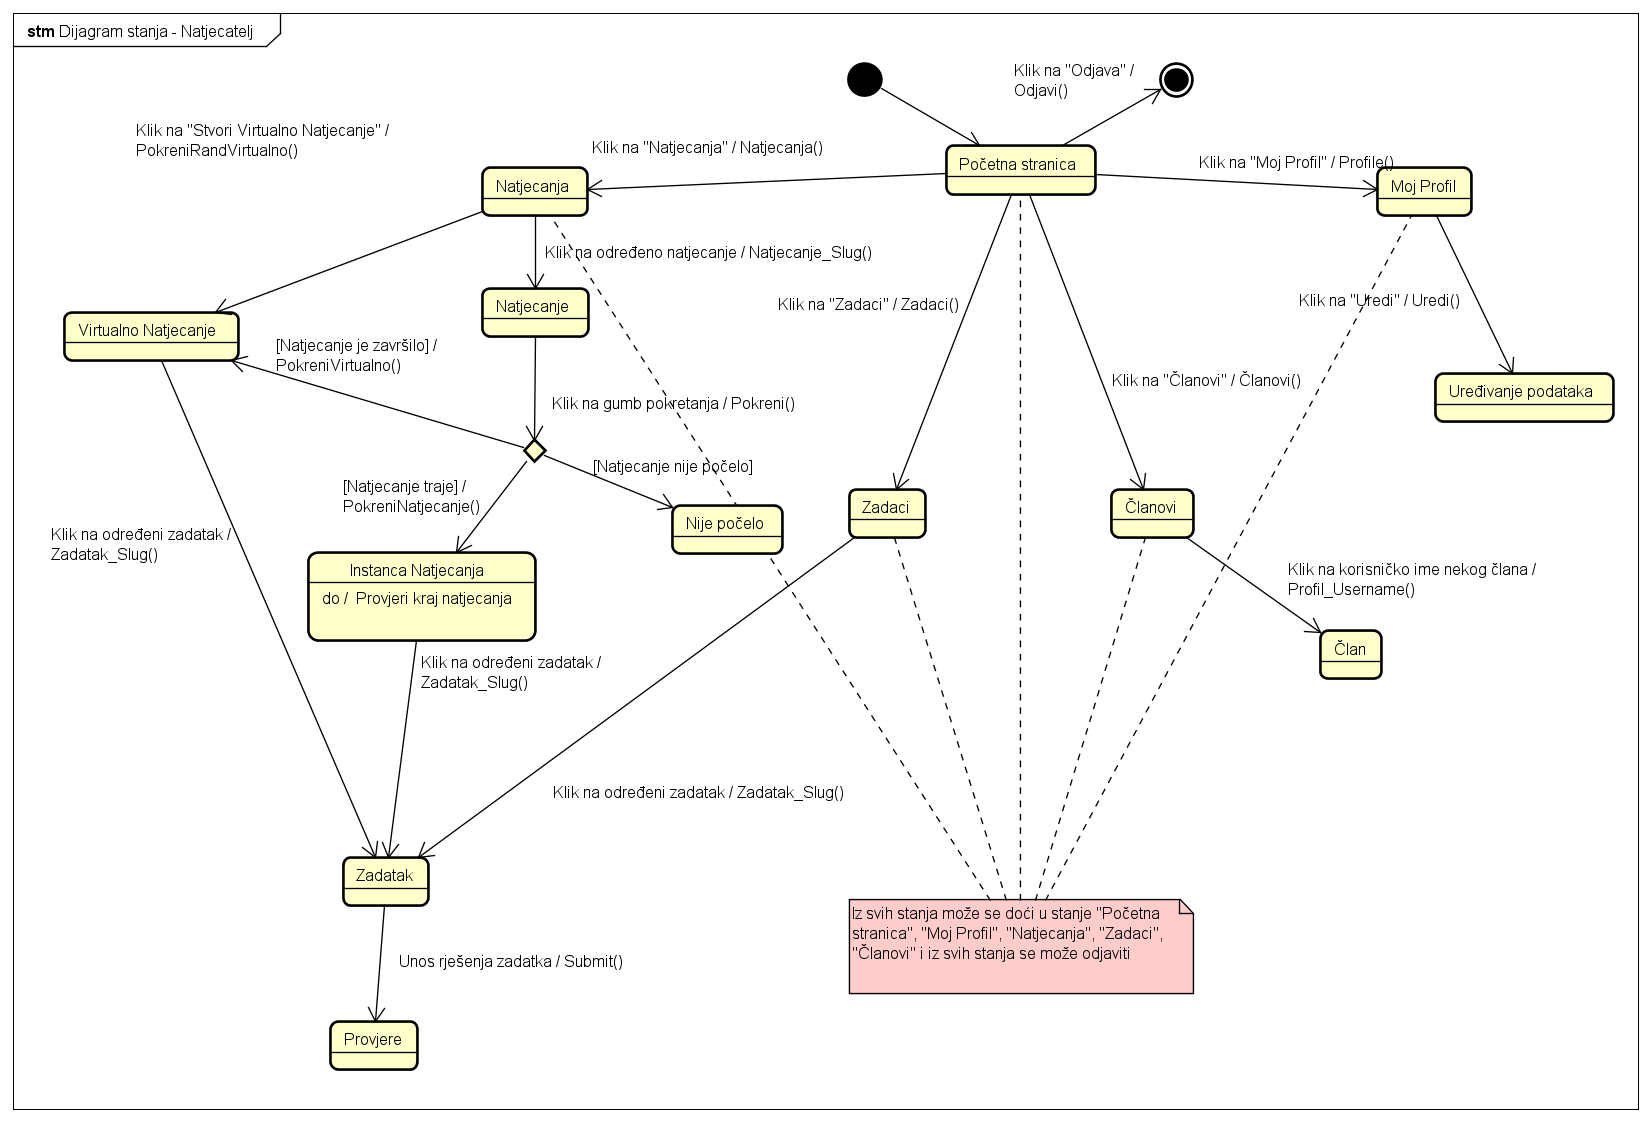
\includegraphics[width=\textwidth]{slike/DijagramStanja.png} %veličina u odnosu na širinu linije
				\caption{Dijagram stanja}
				\label{fig:DijagramStanja} %label mora biti drugaciji za svaku sliku
			\end{figure}
			
			
			\eject 
		
		\section{Dijagram aktivnosti}
			
			Dijagram aktivnosti primjenjuje se za opis modela toka upravljanja ili toka podataka. Ne upotrebljava se za modeliranje događajima poticanog ponašanja. U modeliranju toka upravljanja svaki novi korak poduzima se nakon završenog prethodnog, a naglasak je na jednostavnosti. Na dijagramu aktivnosti 4.4 prikazan je proces rješavanja zadatka. Korisnik se prijavi u sustav, odabere stranicu sa zadacima te odabere željeni zadatak. Prikažu mu se podaci od odabranog zadatka te prostor za unos rješenja. Nakon unosa svojeg rješenja prikaže mu se njegova prolaznost i vrijeme izvođenja.
			
			\begin{figure}[H]
				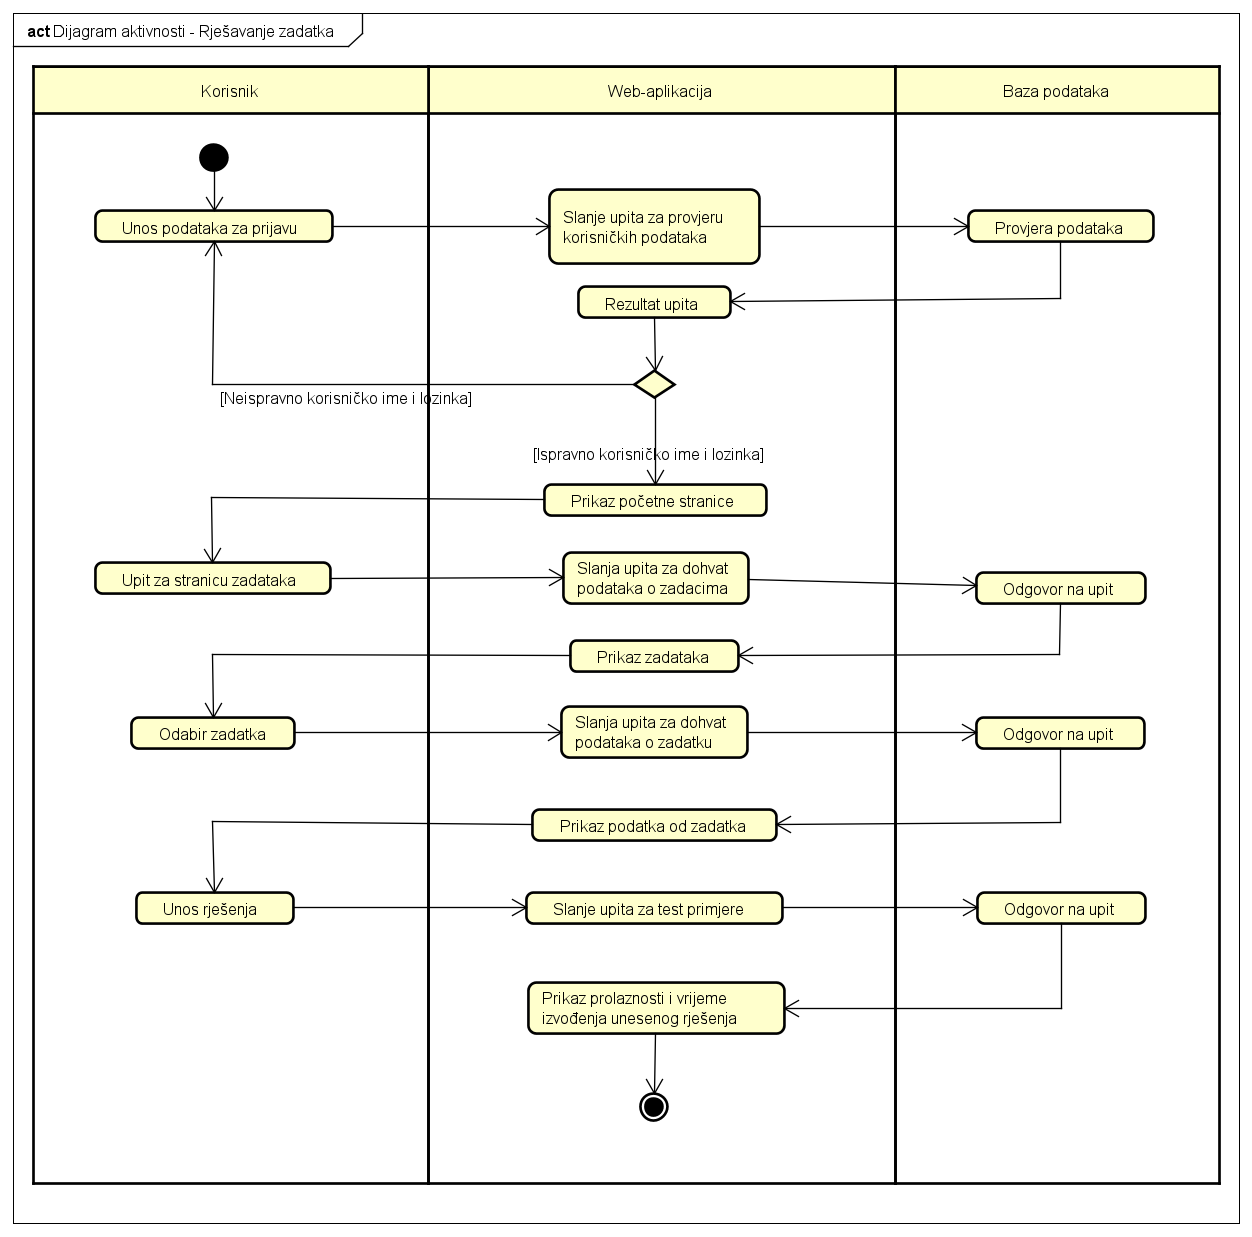
\includegraphics[width=\textwidth]{slike/DijagramAktivnosti.png} %veličina u odnosu na širinu linije
				\caption{Dijagram aktivnosti}
				\label{fig:DijagramAktivnosti} %label mora biti drugaciji za svaku sliku
			\end{figure}
						
			\eject
		\section{Dijagram komponenti}
		
		Dijagram komponenti prikazan na slici 4.5 opisuje organizaciju i međuovisnost komponenti, interne strukture i odnose prema okolini. Sustavu se pristupa preko dva različita sučelja. Preko sučelja za dohvat HTML, CSS i JS datoteka poslužuju se datoteke koje pripadaju frontend dijelu aplikacije. Router je komponenta koja na upit prema specifičnom URL-u određuje koje komponente će se poslužiti na sučelje. Frontend aplikacije sastoji se od detaljno rastavljenih komponenata koje su hijerarhijski organizirane kako bi omogućile jednostavno ponovno iskorištavanje postojećih komponenti te čitljivost koda. Sve JavaScript datoteke ovise o React biblioteci koju koriste za interakciju sa korisničkim preglednikom \\
		
		Preko REST API se šalju zahtjevi na endpointove, koji pozivaju posebne klasne funkcije.  Većina tih funkcija dohvaća ili šalje SQL upite. Posebni wrapper PGDB dobiva od funkcija kombinaciju querya i podataka, priprema ih i šalje zahtjev u SQL bazu podataka. Od baze dobiva podatke, PGDB wrapper ih otpakirava iz tuple-ova i šalje nazad funkcijama koje ih vraćaju REST API-u.
		
			\begin{figure}[H]
				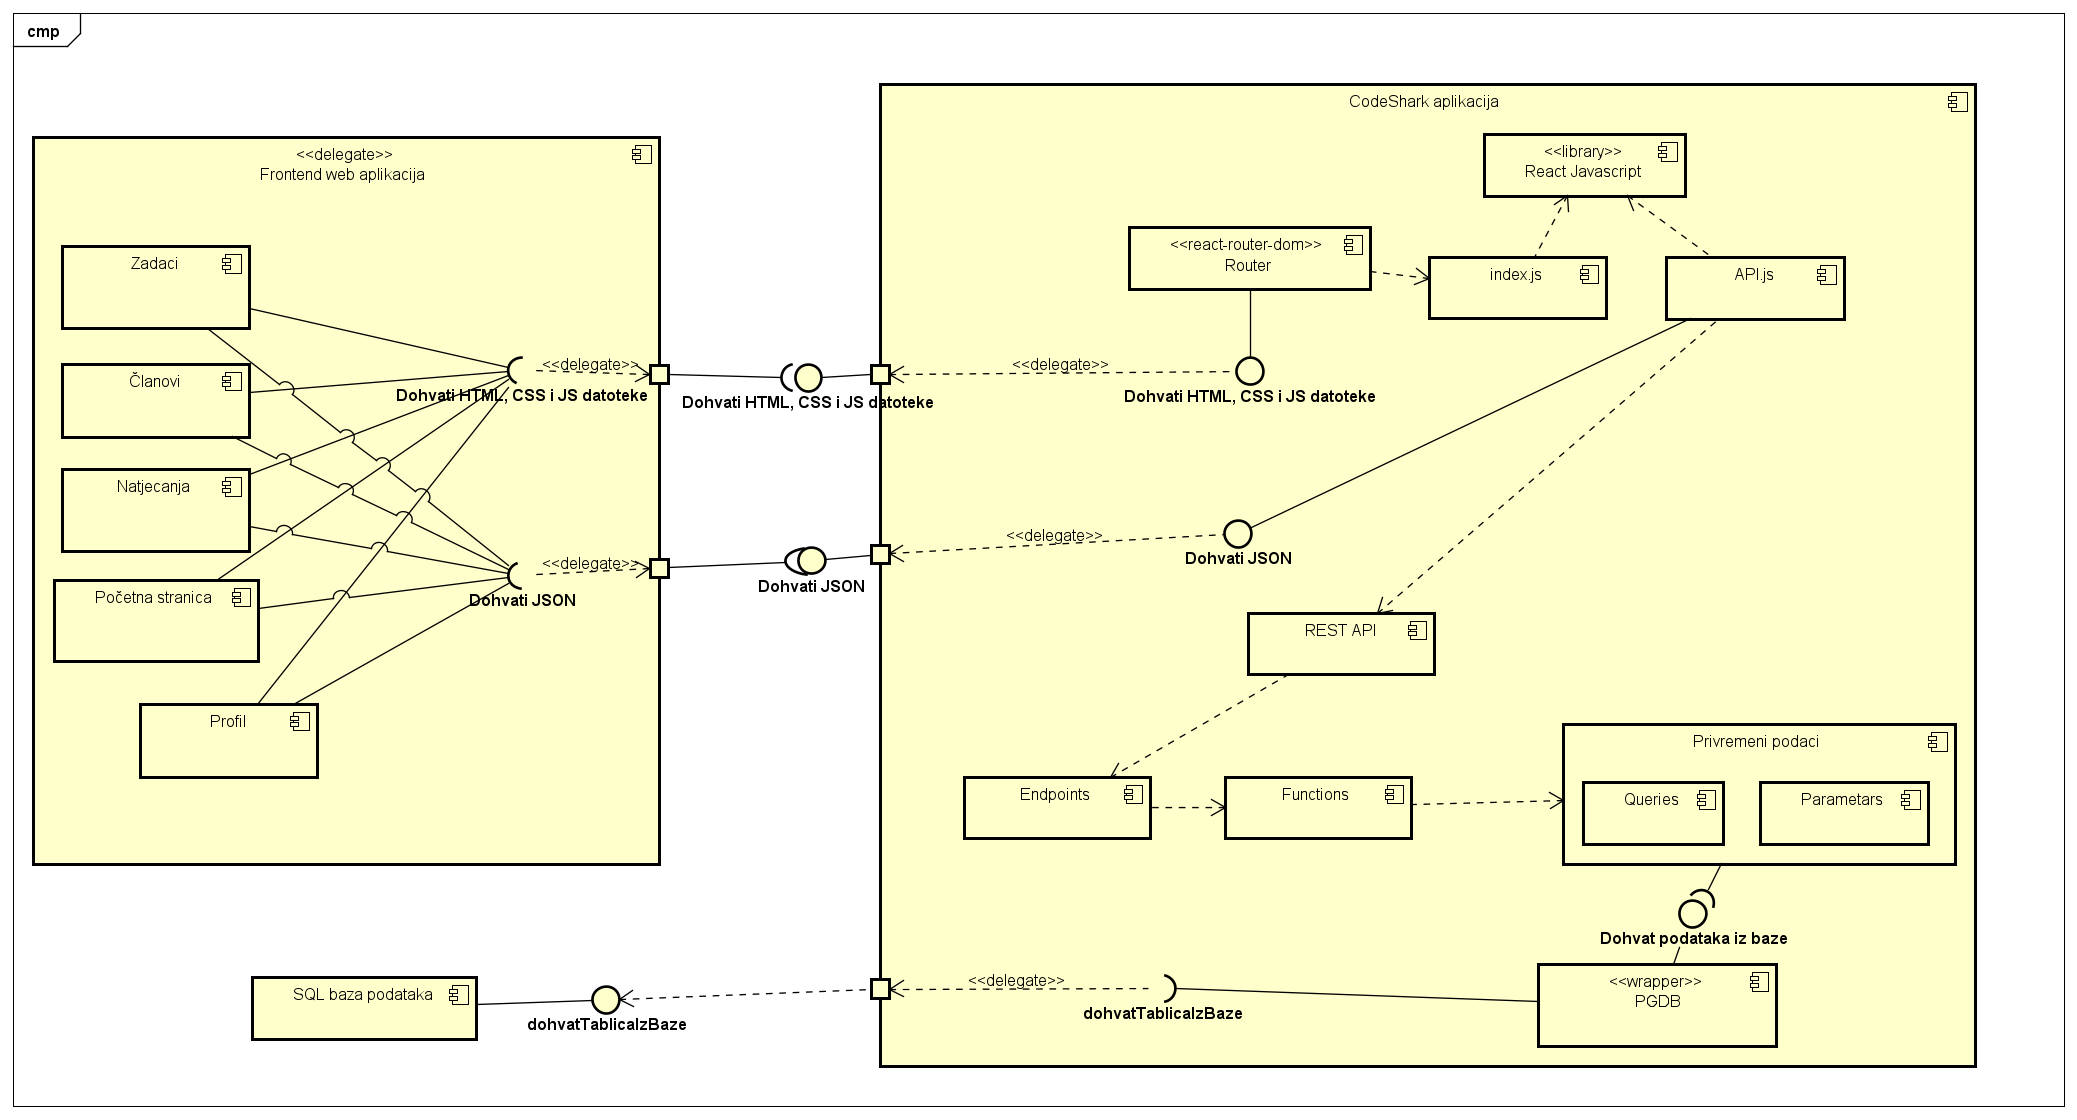
\includegraphics[width=\textwidth]{slike/DijagramKomponenti.png} %veličina u odnosu na širinu linije
				\caption{Dijagram komponenti}
				\label{fig:DijagramKomponenti} %label mora biti drugaciji za svaku sliku
			\end{figure}